\section{Durchführung}
\label{sec:Durchführung}

\subsection{Wheatstone Brücke}
\begin{figure}[H]
    \centering
        \centering
        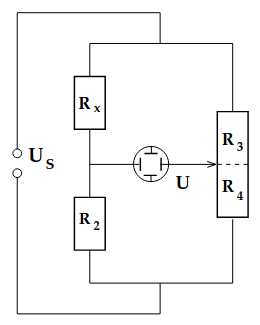
\includegraphics[width=0.35\textwidth]{Bilder/wheatstone.png}
        \caption{Wheatstone Brücke. \cite{anleitung}}
    \hfill
    \label{fig:f2}
\end{figure}
\noindent Bei der Wheatstone Brücke befinden sich nur Ohmsche Widerstände in 
dem Schaltkreis. Dabei sind $R3$ und $R4$ am Potentiometer (Spannungsteiler, 
an dem ein Schleifkontakt über den Widerstandtsdraht gelegt wird, was es
ermöglicht, den Widerstand kontinuierlich einzustellen). Um nun den unbekannten 
Widerstand $R_x$ durch die Kompensationsmethode zu bestimmen, gilt
\begin{equation}
    \label{eqn:1}
    R_x = R_2 \frac{R_3}{R_4}.
\end{equation}
\noindent Als Einstellungen werden folgende Werte genommen:
\begin{align*}
    \label{eqn:werte1}
    \text{Spannungsteiler } R_3 \text{ und } R_4 &= 1\,k\Omega \\
    \text{Frequenz } \nu &= 1\,kHz \\
    \text{Amplitude } U_S &= 1\,V \\
    \text{Widerstand } R_2 &= 332;\, 664;\, 1000\,\Omega \\
\end{align*}


\subsection{Kapazitätsmessbrücke}
\begin{figure}[H]
    \centering
        \centering
        \includegraphics[width=0.35\textwidth]{Bilder/kapazitätsmess.png}
        \caption{Kapazitätsmessbrücke. \cite{anleitung}}
    \hfill
    \label{fig:f3}
\end{figure}
\noindent Da in diesem Bereich des Experiments Kapazitäten bestimmt werden sollen, 
muss der Wechselstrom verwendet weren. Nun werden zwei Potentiometer verwendet, 
das erste wird wie gehabt als Spannungsteiler für $R3$ und $R4$ verwendet. Das 
zweite Poti wird als Spannungsteiler für die unbekannten Komponenten $C_x$ mit 
$R_x$ und der bekannten Kapazität $C_x$ genutzt.
\par\vspace{0.5em}
Die Brücke wird nun abgeglichen, indem alternierend an dem Poti ein Minimum 
eingestellt wird und an dem Anderen die Spannung am Oszilloskop minimiert wird.
Dieses Verfahren wird so häufig wiederholt, bis die Brücke abgeglichen ist.
Für den Widerstand gilt weiterhin
\begin{equation}
    R_x = R_2 \frac{R_3}{R_4}.
\end{equation}
Für die zu bestimmende Kapazität dann:
\begin{equation}
    \label{eqn:2}
    C_x = C_2 \frac{R_4}{R_3}.
\end{equation}
\noindent Als Einstellungen werden folgende Werte genommen:
\begin{align*}
    \label{eqn:werte1}
    \text{Kapazität } C_2 &= 450;\, 597;\, 992\, nF \\
    \text{Frequenz } \nu &= 1\,kHz \\
    \text{Amplitude } U_S &= 1\,V \\
\end{align*}

\subsection{Induktivitätsmessbrücke}
\begin{figure}[H]
    \centering
        \centering
        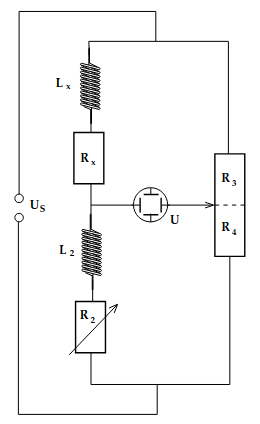
\includegraphics[width=0.35\textwidth]{Bilder/induktivitaetsmess.png}
        \caption{Induktivitätsmessbrücke. \cite{anleitung}}
    \hfill
    \label{fig:f4}
\end{figure}
\noindent Der Aufbau erfolgt analog zu dem der zuvor angesprochenen 
Kapazitätsmessbrücke. Es werden lediglich Kondensatoren mit Spulen ausgewechselt.
Folglich wird wieder der Aufbau mit Wechselstrom betrieben. Für den Serienwiderstand 
gilt erneut \autoref{eqn:1}. Eine Gleichung für die Induktivität ergibt sich 
analog zu \autoref{eqn:2}:
\begin{equation}
    \label{eqn:3}
    L_x = L_2 \frac{R_4}{R_3}.
\end{equation}

\subsection{Wien-Robinson Messbrücke}
\begin{figure}[H]
    \centering
        \centering
        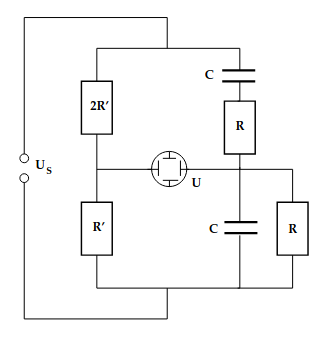
\includegraphics[width=0.35\textwidth]{Bilder/wien_robinson.png}
        \caption{Wien-Robinson Messbrücke. \cite{anleitung}}
    \hfill
    \label{fig:f5}
\end{figure}
Bei dieser Brücke, dessen Aufbau in \autoref{fig:f5} dargestellt ist, soll der 
Frequenzgang und der Klirrfaktor der Speisespannung ermittelt werden. Letzteres 
ist als Maß für die Qualität einer Spannungsquelle, insbesondere in Bezug auf 
die Reinheit der ausgegebenen Sinunsspannung, zu versethen; er gibt an, wie 
stark die erzeugte Spannung von einer Sinurkurve abweicht. Gegensätzlich zu 
den vorherigen Versuchen wird diese Brücke nicht zur Messung von Komponenten 
genutzt, alle Komponenten verfügen über bekannte Werte. Die Brücke dient als 
elektronischer Filter für die Frequenz. Für das Verhältnis von Brückenspannung 
$U_{Br}$ zu der Speisespannung $U_S$ gilt:
\begin{equation}
    \left|\frac{U_{Br}}{U_S}\right|^2 = \frac{(\omega ^2 R^2 C^2 -1)^2}{9((1-R^2 C^2)^2+9 \: \omega ^2 R^2 C^2)}
\end{equation}
Bei Abgleichung der Brückenspannung (links) und der normierten Frequenz (rechts)
\begin{equation}
    \begin{aligned}
        \omega_0 &= \frac{1}{RC}, & \Omega &= \frac{\omega}{\omega_0}
    \end{aligned}
\end{equation}
reduziert sich das Verhältnis auf 
\begin{equation}
    \label{eqn:omega}
    \left|\frac{U_{Br}}{U_S}\right|^2 = \frac{9(\Omega ^2 -1)^2}{9(1-\Omega^2)^2+81 \: \omega ^2 \Omega^2}.
\end{equation}
Bei dieser Gleichung handelt es sich um einen Filter, welcher bei der Frequenz 
$\omega=\omega_0$ sperrt, sodass keine Brückenspannung mehr dokumentiert werden 
kann. Sollte dieser Idealfall nicht eintreten, so kommt der Klirrfaktor ins Spiel, 
die Oberwellen der Speisespannung führen zu einer detektierbaren Brückenspannung.
Der Anteil dieser Wellen wird durch eben diesen Klirrfaktor $k$ bestimmt. Dieser 
lautet
\begin{equation}
    \label{eqn:Klirrfaktor}
    k = \frac{\sqrt{\sum\limits_{i=2}^N U_i^2}}{U_1}
\end{equation}
mit der Amplitude der Grundwelle $U1$ und den Amplituden der i-ten Oberwellen 
$U_i$. Je näher der Klirrfaktor an dem Wert Null ist, desto weniger Oberwellen 
werde erzeugt.